\documentclass{article}

\usepackage[russian]{babel}
\usepackage{listings}
\usepackage{pgfplots}
\usepackage{amsfonts}

\usepackage[a4paper,top=2cm,bottom=2cm,left=3cm,right=3cm,marginparwidth=1.75cm]{geometry}

\usepackage{amsmath}
\usepackage{graphicx}
\usepackage[colorlinks=true, allcolors=blue]{hyperref}

\definecolor{codegreen}{rgb}{0,0.6,0}
\definecolor{codegray}{rgb}{0.5,0.5,0.5}
\definecolor{codepurple}{rgb}{0.58,0,0.82}
\definecolor{backcolour}{rgb}{0.95,0.95,0.92}

\lstdefinestyle{mystyle}{
    backgroundcolor=\color{backcolour},
    commentstyle=\color{codegreen},
    keywordstyle=\color{magenta},
    numberstyle=\tiny\color{codegray},
    stringstyle=\color{codepurple},
    basicstyle=\ttfamily\footnotesize,
    breakatwhitespace=false,
    breaklines=true,
    captionpos=b,
    keepspaces=true,
    numbers=left,
    numbersep=5pt,
    showspaces=false,
    showstringspaces=false,
    showtabs=false,
    tabsize=2
}

\title{Отчёт о выполнении практического задания}
\author{Владислав Лазар, 204 группа}

\begin{document}
\maketitle

\section{Цели работы}
\begin{enumerate}
    \item Ознакомиться на практике с методами оценивания параметров распределения
    \item Используя свойства модели, вычислить для неё информацию Фишера
    \item Составить оценку для полученной функции от параметра и проверить её точность
\end{enumerate}

\section{Постановка задачи}

Дана модель - гамма распределение $\Gamma(\theta, 1.5)$. Для данной модели найти информацию Фишера $i(\theta)$, построить выборку размерности 1500 и, используя  некоторую оценку параметра $\theta$, оценить значения функции информации и проверить погрешность оценивания.

\section{Выполнение задания}
\subsection{Нахождение $i(\theta)$}

Для произвольного распределения $i(\theta)$ информация Фишера равна $i(\theta) = \mathbb{E}_{\theta}(\frac{\partial \ln{f(\xi, \theta)}}{\partial \theta})^2$, где $f(x, \theta)$ - плотность распределения. В нашем случае плотность равна $f(x, \theta) = \frac{\sqrt(x)e^{-\frac{x}{\theta}}}{\Gamma(\frac{3}{2})\theta^{\frac{3}{2}}}$.
Найдём сначала $\frac{\partial\ln{f(x, \theta)}}{\partial \theta}$:

$\frac{\partial\ln{f(x, \theta)}}{\partial \theta} = \frac{\Gamma(\frac{3}{2})\theta^{\frac{3}{2}}}{\sqrt{x}e^{-\frac{x}{\theta}}} \frac{e^{-\frac{x}{\theta}} \frac{x}{\theta^2} \theta^{\frac{3}{2}} - e^{-\frac{x}{\theta}}\frac{3}{2} \sqrt{\theta}}{\theta^3} \frac{\sqrt{x}}{\Gamma(\frac{3}{2})} = \theta^{\frac{3}{2}} \frac{x\theta^{-\frac{1}{2}} - \frac{3}{2} \sqrt{\theta}}{\theta^3} = \frac{x\theta - \frac{3}{2}\theta^2}{\theta^3} = \frac{x}{\theta^2} - \frac{3}{2\theta}$. \newline
Тогда $i(\theta) = \mathbb{E}_{\theta}(\frac{x}{\theta^2} - \frac{3}{2\theta})^2 = \mathbb{E}_{\theta} (\frac{x^2}{\theta^4} - \frac{3x}{\theta^3} + \frac{9}{4\theta^2}) = \frac{9}{4\theta^2} - \frac{3}{\theta^3} \mathbb{E}_{\theta}(x) + \frac{1}{\theta^4} \mathbb{E}_{\theta}(x^2)$. \newline \newline
Так как $\mathbb{D}_{\theta}(x) = \mathbb{E}_{\theta}(x^2) - \mathbb{E}^{2}_{\theta}(x)$,  $\mathbb{D}_{\theta}(x) = \frac{3}{2}\theta^2$ , $\mathbb{E}_{\theta}(x) = \frac{3}{2}\theta$, то:
\newline \newline
$i(\theta) = \frac{3}{2\theta^2}$

\subsection{Построение оценки для $\theta$}

Для оценивания неизвестного параметра воспользуемся формулой матожидания: $\mathbb{E} = \frac{3}{2} \theta$. Поскольку матожидание хорошо аппроксимируется средним арифметическим выборки, то используем следующую оценку: \newline
$\widetilde{\theta} = \frac{2\overline{\mathbb{X}}}{3}$

\subsection{Использование программных средств}

Для программной реализации был выбран язык Python и следующий набор библиотек: numpy, matplotlib. Для генерации выборки использовалась функция np.random.gamma. Данная генерирует необходимую нам выборку, вот, например, гистограмма построенной выборки при $\theta = 1$:

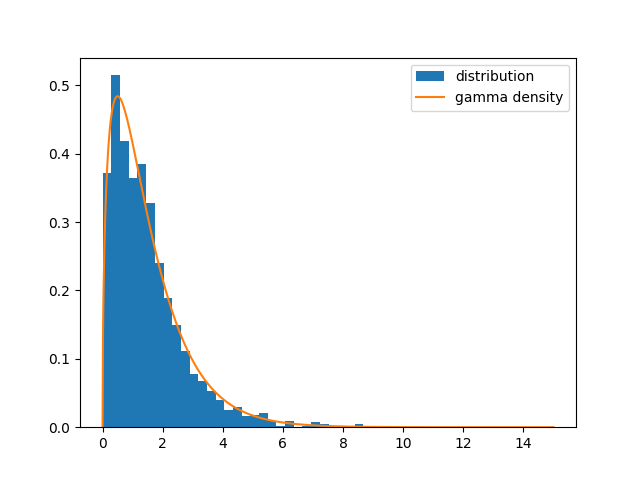
\includegraphics[scale=0.5]{gamma.png}

Как видно, выборка действительно распределена в соответствии с нужным законом.


\subsection{Текст программы}

\lstset{style=mystyle}
\begin{lstlisting}[language=Python]
import numpy as np
import matplotlib.pyplot as plt
import math


def gamma_density(x: np.array, theta: float) -> float:
    return (x ** 0.5 * np.exp(-x / theta)) / (math.gamma(1.5) * theta ** 1.5)


def param_plot(theta: float) -> None:
    x = np.linspace(0, 15, 1000)
    y = gamma_density(x, theta)
    plt.plot(x, y, label='gamma density')


def info(theta: float, a: float) -> float:
    return a / theta ** 2


def i_est(X: np.ndarray, a: float) -> float:
    theta_est = np.mean(X) / a
    return a / theta_est ** 2


def main():
    accuracy = []
    params = np.linspace(0.7, 15, 50)
    true_info = []
    estimates = []
    for theta in params:
        n = 1500
        a = 1.5
        X = np.random.gamma(a, theta, n)
        i = info(theta, a)
        i_e = i_est(X, a)
        true_info.append(i)
        estimates.append(i_e)
        print(i, i_e, abs(i - i_e) / i * 100)
        accuracy.append(abs(i - i_e) / i * 100)
    plt.plot(params, true_info, color='red', label=r'i($\theta$)')
    plt.plot(params, estimates, color='blue', label='estimates')
    plt.legend()
    plt.show()
    print(100.0 - np.mean(accuracy))

main()
\end{lstlisting}

\subsection{Полученные реультаты}

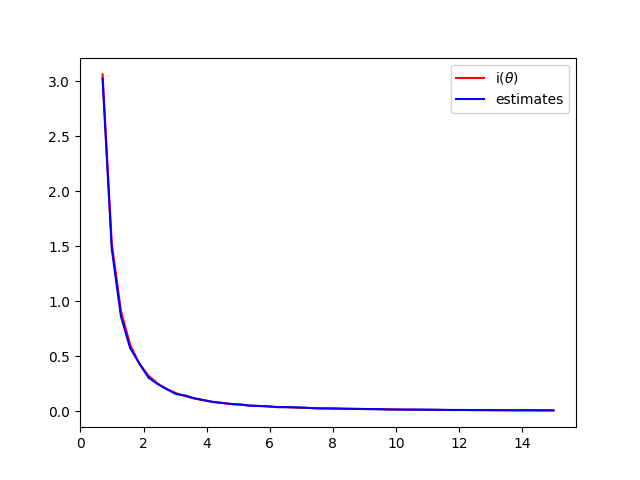
\includegraphics[scale=0.5]{plot_full.png}

Из-за масштаба графики довольно плохо различимы, поэтому было принято решение произвести аналогичные вычисления на меньшем отрезке:

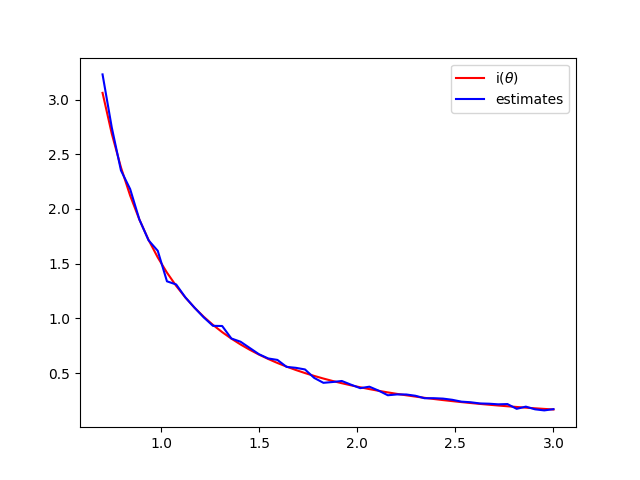
\includegraphics[scale=0.5]{myplot.png}

Как можно видеть, оценка довольно точно приближает значение параметра. Судя по отладочному выводу, относительная погрешность оценки всего раз превысила 10\%. Таким образом, можно заключить, что оценка является достаточно точной для практического применения.

\section{Вывод}

Для распределения $\Gamma(\theta, 1.5)$ получена оценка, приближающая второй параметр с точностью ~96.68\% (если брать в качестве точности среднее значение точности для каждого значения параметра). Такой оценкой является $\widetilde{\theta} = \frac{2\overline{\mathbb{X}}}{3}$. При использовании этой оценки для вычисления информации Фишера на больших отрезках для параметра графики функций почти сливались, что говорит о соответствии заявленной точности.

\end{document}